%%%%%%%%%%%%%%%%%%%%%%%%%%%%%%%%%%%%%%%%%%%%%%%%%%%%%%%%%%%%%%%%%%%%%%%%
\chapter{Diseño}
\label{ch:diseno}
%\fxnote{Puede resultar conveniente cambiar el título a ``Diseño'' dado
 % que no existe un capítulo de análisis el salto desde requisitos a
 % arquitectura parece excesivo.}

%\fxnote{Mete un label en cada capítulo para poder referirnos a él.}

En este capítulo se presentará el diseño de la aplicación. Para un mejor entendimiento explicaremos brevemente el diseño interno de un dispositivo iOS conocido técnicamente como Cocoa Touch. Seguiremos por una breve descripción del API de acceso a los servicios de Betfair y concluiremos con una explicación detalla de la arquitectura desplegada en la aplicación.


\section{Descripción general}
 
  El análisis de los requisitos presentados en el capítulo \ref{ch:requisitos} %\fxnote{meter el label en el capítulo adecuado}
   dará como resultado la arquitectura de la aplicación. Para llevar a cabo su desarrollo, hemos tenido en cuenta la arquitectura del dispositivo y las herramientas adjuntas para el desarrollo de aplicaciones. Todas las decisiones tomadas en la construcción de la arquitectura de la aplicación se han basado en los límites o restricciones impuestas por el uso de la arquitectura de Apple y los límites impuestos en el uso del API de Betfair. Para comprender mejor el diseño de la aplicación expondremos brevemente la arquitectura impuesta por Apple en el iPhone y la tecnología en la que se basa el API que ofrece Betfair para el uso de sus servicios.

\section{API de iPhone/iPod Touch: Cocoa Touch}
 La arquitectura del terminal móvil se basa en su sistema operativo \emph{iOS} de Apple. Este sistema operativo, a grandes rasgos, es un subconjunto del sistema operativo que llevan los ordenadores personales de Apple. Esta decisión favorece el desarrollo de aplicaciones para sus plataformas. Simplifica la tarea a los desarrolladores de aplicaciones de ordenadores de sobremesa de Apple de programar aplicaciones móviles sin necesidad de aprender un lenguaje o arquitectura totalmente nueva.
 
 El iOS es capaz de ejecutar dos tipos de aplicaciones: 
\begin{itemize}
\item Aplicaciones nativas: 
aquellas aplicaciones que usan bibliotecas del sistema para su ejecución. 
\item Aplicaciones web: desarrollos basados % \fxnote{por?} 
en lenguajes de programación de páginas web y sólo se ejecutan al acceder por el navegador de Internet del dispositivo. Sorprende la capacidad de ciertos desarrolladores para generar aplicaciones con un look\&feel muy parecido a las aplicaciones nativas. Por supuesto, para su ejecución requieren de una conexión de datos hacia Internet.
 \end{itemize}

 %\fxnote{La introducción de gráficos o figuras puede hacerse de dos
  % formas: o la ``empotras'' directamente como he hecho yo con la
   %figura de las capas del OS o la metes en un entorno ``figure'' y la
   %referencias con un ``ref'' como he hecho con la figura \ref{fig:API
    % Betfair}, lo que creas más conveniente}

\noindent
La siguiente figura muestra la estructura de capas del iOS:

%\begin{center}
%  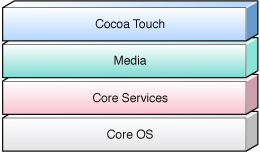
\includegraphics[width=0.5\textwidth]{./images/overview_systemlayers.jpg}
%\end{center}

\begin{figure} [h]
  \centering
    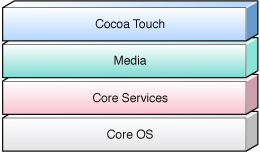
\includegraphics[width=0.6\textwidth]{./images/overview_systemlayers.jpg}
  \caption{Capas del iOS}
  \label{fig:Capas-del-iOS}
\end{figure}

En la parte baja del sistema se encuentran las capas encargadas de los
servicios fundamentales que permiten la ejecución de las aplicaciones,
y en las superiores contienen las capas sobre los servicios multimedia
y de las más altas tecnologías.
 

A continuación expondremos una breve descripción de cada capa:

%\fxnote{He cambiado el entorno ``itemize'' a ``description'' para que
 % veas como queda, si te gusta lo mantienes, si no lo cambias. También
 % he modificado la indentación en el código fuente de latex para que
 % veas que se pueden meter cambios de linea sin probleamas (dos
 % cambios de linea consecutivos = nuevo párrafo).}

\begin{description}
\item[Core OS.]  Es la capa que contiene el núcleo de
  sistema (\emph{kernel}) %\fxnote{Recuerda, inglés enfatizado, al
   % menos en la primera aparición, encárgate tú del resto.},
  , los controladores para dispositivos internos y las interfaces básicas del sistema
  operativo. El kernel es el responsable de todos los aspectos
  relacionados con el sistema operativo. Es el encargado de gestionar
  la memoria virtual, \emph{threads} (procesos ligeros), sistema de ficheros,
  red y procesos de comunicación. Los controladores son los encargados
  de proporcionar la interfaz entre el \emph{hardware} y los \emph{frameworks} de
  las capas superiores.
\item[Core Services.] Es la capa responsable de proporcionar los
  servicios básicos del sistema a las aplicaciones para su uso. En
  ella encontramos el acceso a la agenda del dispositivo, la gestión
  de estructura de datos, la gestión de las interfaces de red, la
  gestión de la localización del dispositivo, la gestión de la seguridad
  del sistema y el soporte para bases de datos SQL y XML.
\item[Media.] Es la capa encargada de dar soporte a las
  tecnologías de gráficos y al audio y video para proporcionar al usuario
  los medios multimedia vistos en un dispositivo móvil.
  %\fixme{No marketing, please.}. 
  Aún más importantes que las tecnologías
  en sí, es el hecho de que esta capa fue diseñada para facilitar al desarrollador su uso
  para crear aplicaciones con una gran apariencia en su interfaz de
  usuario y una reproducción de audio. %\fixme{No marketing.}.
\item[Cocoa Touch.]  Es una de las capas más importantes del iOS
  para un desarrollador. %\fxnote{desde el punto de vista del desarrollador, supongo}. 
  Es la encargada de proveer los objetos básicos necesarios para la
  implementación de aplicaciones. La puerta de acceso de los desarrolladores
  para el uso de los servicios de las anteriores capas.
\end{description}

%\fixme{El siguiente párrafo no se entiende bien, al menos yo no lo
  %entiendo bien del todo.}
  
  Esta última capa es la que diferencia la plataforma móvil de la plataforma PC en los entornos de Apple. Es el API que nos ofrece %\fxnote{ofrece-ofrece} 
  Apple para el uso de las tecnologías asociadas a un dispositivo móvil, especialmente en el uso de la tecnología táctil. En ella podemos encontrar los siguientes frameworks%\fxnote{¿es la footnote una definición de ``framework''?}
  \footnote{Un framework es una estructura de soporte definida, en la cual otro proyecto de software puede ser organizado y desarrollado.}: 

%\fxnote{Probablemente usaría description en vez de itemize.}

 \begin{description}
 	\item [UIKit.] Contiene todas las clases necesarias para la programación de la interfaz de usuario de las aplicaciones así como el acceso a las principales tecnologías hardware % \fxnote{no me gusta el palabro ``tecnologías físicas''}
	 propias del dispositivo  móvil:
		 \begin{itemize}
 			\item soporte para copiar, cortar y pegar.
 			\item soporte para la creación de gráficos y ventanas del sistema.
 			\item soporte para la gestión de eventos \emph{multitouch} y eventos realizados al pulsar la pantalla con más de un dedo.
			 \item soporte para la creación de contenido tanto de texto como de web.
 			\item soporte para la creación de controles y objetos del sistema.
 			\item soporte para la accesibilidad de aplicaciones.
 			\item soporte para el acceso a las capacidades hardware del dispositivo: batería, cámara, acelerómetros, sensor de proximidad \ldots 
 		\end{itemize}
 	 \item [Foundation.] Es un \emph{framework} heredado de la plataforma OS X. Provee el soporte para las siguientes funcionalidades: % \fxnote{funcionalidades mejor?}:
 		\begin{itemize}
			\item colecciones de datos (arrays, sets \ldots)
			\item gestión del tiempo y fechas.
			\item gestión de las preferencias del dispositivo.
			\item gestión de URLs.
			\item internacionalización del dispositivo.
		\end{itemize}
	\item [Address Book UI.] Una de las partes más importantes en un dispositivo móvil es la agenda de contactos. Nos proporciona las herramientas necesarias para gestionar toda la interfaz de usuario relacionado con el acceso a los contactos del dispositivo.
	\item [Message UI.] Proporciona el soporte necesario para componer y gestionar mensajes de correo electrónico en nuestras aplicaciones.
	\item [Map kit.]  Esta interfaz proporciona la creación de una vista de un mapa geográfico escalable con posibilidad de incrustar en él información detallada. Un típico ejemplo es la localización en un mapa de un restaurante.
	\item [Game Kit.] Nos permite añadir a nuestras aplicaciones el soporte de comunicaciones \emph{peer-to-peer} o redes dos a dos. Especialmente importante en aplicaciones  o juegos multiusuario.
	\item [Push Notification Service.] Proporciona un camino para notificar a los usuarios que una aplicación tiene nueva información relevante. El sistema notifica al usuario la información incluso si la aplicación no está en ejecución.

\end{description}

 Para poder desarrollar aplicaciones para dispositivos iOS, Apple pone a disposición de forma gratuita un conjunto de herramientas de desarrollo (SDK) que se encuentra disponible en su portal web. %\fixme{No entiendo.}

%PACO CAMBIA ESTO 
\begin{afixme}
  Entiendo que la parte más importante, en lo que afecta a la  aplicación, de todo lo que has contado es el UKit y quizá algo del Foundation. Tendrás que hablar en algún momento sobre en qué forma influye en la arquitectura final y porqué y para ello es probable que antes ofrezcas algún dato extra sobre sus típicos usos, incluso algún ejemplo. No lo tengo claro, estoy pensando en el lector y aún no he leído el resto así que puedo estar equivocándome.
\end{afixme}

\section{Arquitectura del API de Betfair}

	El API de Betfair está diseñado bajo un protocolo \emph{SOAP}\footnote{Simple Object Access Protocol: es un protocolo estándar que define cómo dos objetos en diferentes procesos pueden comunicarse por medio de intercambio de datos XML.} % CAMBIA ESTO
	\fixme{Esto hay que solucionarlo mediante una referencia bibliográfica utilizando bibtex, pregunta si no sabes cómo y lo vemos juntos.} que esta disponible a través de una conexión web HTTPS\footnote{Hypertext Transfer Protocol Secure segura.} \fxnote{Lo mismo}.  

%\fixme{Creo que se hace fundamental explicar en qué consiste todo este asunto del WSDL, cómo se usa (probablemente hay varios ``workflows'' posibles), un par de ejemplos pueden ser determinantes para entender la filosofía. En estos %momentos, como lector, estoy más interesado en que me cuentes cómo se materializa ese API que en ningún otra cosa. También puedes dar el ejemplo un poco más adelante y avisar al lector. Puedes utilizar subsections para organizar %bien la exposición.}

          El API está disponible a partir de un fichero en formato WSDL\footnote{Web Services Description Language, un formato XML que se utiliza para describir servicios Web.} en el portal de desarrolladores de Betfair. Dicho formato describe la interfaz para todos los servicios web disponibles de Betfair. Un programa cliente que se conecta a un servicio web puede leer el WSDL para determinar qué funciones están disponibles en el servidor. Los tipos de datos especiales se incluyen en el archivo WSDL en forma de XML. El cliente puede usar SOAP para hacer la llamada a una de las funciones listadas en el WSDL. En el capítulo \ref{ch:implemetacion} describiremos cómo hemos hecho uso de este fichero para construir las llamadas al servidor y consumir dichos servicios de Betfair.
          
 Los servicios proporcionados por el API se dividen en dos conjuntos: 
          
\begin{itemize}
	\item Global: contiene todas las llamadas referentes a los servicios básicos de Betfair, tales como el inicio de sesión, la administración de tu cuenta Betfair, tus fondos y las llamadas para navegar por los diferentes eventos disponibles en el portal de apuestas.
	\item Exchange: contiene las llamadas a los servicios relacionados con las apuestas, es decir, apostar por un evento, descripción de los mercados disponibles, actualización o cancelación de las apuestas ya realizadas, historial de todas nuestra apuestas \ldots %\fxnote{usa ldots: \ldots}
\end{itemize}
%\begin{figure} [h]
 % \centering

 % \begin{afixme}
 %   ¿Para qué sirve esta figura?
%  \end{afixme}

    %\includegraphics[width=0.6\textwidth]{./images/DeveloperBetfair.png}
  %\caption{API Betfair}
  %\label{fig:API Betfair}
%\end{figure}

  Para cada conjunto existen dos formas de acceso al API:
\begin{description}
	\item [Free Access API.]  Con este acceso tendremos disponibles los servicios básicos del portal y las herramientas suficientes para poder apostar por los eventos disponibles. Gratuito pero con acceso limitado a las llamadas de los servicios.
	\item [Full Access API.] Acceso de pago donde están disponibles los servicios exclusivos del portal tales como la información avanzada de los mercados, la gestión avanzada de nuestra cuenta de usuario\ldots Se gestiona a partir de una cuota anual y no existen límites en las llamadas a los servicios del API.
\end{description}


%\fixme{Este aspecto creo que es importante y que debe resaltarse en una subsection.}

%\fxnote{Quizá aquí puedes dar más detalles sobre SOAP, WSDL su uso en general y el nuestro en particular.}

    Resaltar en este apartado que dado que nuestra aplicación no soporta la plataforma WSDL, hubo que implementar cada llamada a los servicios de Betfair bajo la tecnología de Apple y su posterior serialización para el tratamiento de datos de la aplicación. Por cada llamada descrita en el archivo de definición de servicios hemos tenido que implementar la estructura de la comunicación mediante mensajes XML\footnote{Extensible Markup Language, es un metalenguaje extensible de etiquetas desarrollado por el World Wide Web Consortium (W3C).}, uno de petición y otro de respuesta con un parser asociado que traduzca dichos mensajes. En el capítulo \ref{ch:implemetacion} veremos con más detalle la adaptación de WSDL a la plataforma iOS.

    Los servicios básicos que hemos usado para el desarrollo de la aplicación han sido:

%\fixme{Yo elegiría una tipografía específica para nombrar cada servicio. Puede bastar con lstinline.}
\begin{itemize}
	\item \lstinline{Login}: 
		llamada para poder usar los servicios web de Betfair. 
	\item \lstinline{GetActiveEventTypes}: 
		con esta llamada obtenemos todos los eventos deportivos actualmente en marcha por los que se puede apostar.
	\item  \lstinline{GetAllMarkets}:
		con esta llamada obtenemos todos los mercados referentes a un evento.
	\item  \lstinline{GetCurrentsBets}:
		llamada por la cual obtenemos todas las apuestas activas que hemos realizado.
	\item  \lstinline{GetMarketPrices}:
		obtenemos los precios (back y lay) actuales por un evento determinado.
	\item  \lstinline{GetMarket}:
		esta llamada nos devuelve todos los datos referentes a un mercado.
	\item  \lstinline{PlaceBets}:
		con esta llamada enviamos una apuesta a Betfair.
	\item  \lstinline{ViewProfile}: 
		esta llamada nos devuelve los datos de perfil de usuario.
	\item  \lstinline{RetrieveLIMBMessage}:
		 con esta llamada obtenemos los mensajes del sistema pendientes de acción por parte del usuario.
\end{itemize}

\section{Arquitectura de la aplicación}
%\fixme{Las comillas en LaTeX se escriben ``así''.}

 Para el diseño de la arquitectura nos hemos basado en el patrón de diseño ``Modelo Vista Controlador (MVC)''. Dicho patrón es muy utilizado en la programación orientada a objetos, donde los objetos del modelo representan los datos de la aplicación y son persistentes. Fundamentalmente consiste en separar los datos de una aplicación, la interfaz de usuario, y la lógica de control en tres componentes distintos:
 
 
 \begin{description}
 	\item [Modelo.] Es la representación de toda la información con la cual el sistema trabajará. El modelo es independiente de cualquier representación o vista.
	\item [Vista.] Se encarga de presentar el modelo en un formato adecuado para interactuar, normalmente mediante una interfaz de usuario.
	\item [Controlador.] Se encarga de responder a eventos. Esto implica cambios en el modelo y en la vista.
\end{description}
 
  La razón del uso de este patrón se debe a dos cuestiones fundamentales:
\begin{itemize}
	\item La facilidad entre la comunicación del %\fxnote{entre-entre?}
	modelo de datos y la interfaz. Añadir también que cualquier cambio en la interfaz de usuario no afecta al resto del modelo, por lo que se gana en facilidad a la hora de seguir desarrollando la solución en el futuro.
	\item Apple, en el uso de las herramientas de desarrollo del SDK, recomienda el uso de dicho patrón para la creación de la interfaz de usuario de la aplicación. Esta recomendación es debido a la arquitectura interna del iOS y a que sus herramientas de desarrollo también están orientadas a esta solución.
	\item La estructura jerárquica de los datos obtenidos a través del API de Betfair. Este patrón nos facilita la representación de los mismos.
\end{itemize}

%\fxnote{MVC es un nombre demasiado genérico y bastante manido, quizás quieras explorar con más profundidad las características exactas del patrón que hayas aplicado: http://www.aspiringcraftsman.com/2007/08/interactive-application-architecture/, http://c2.com/cgi/wiki?MvcIsNotObjectOriented}

\subsection{Núcleo de la aplicación}
	Toda aplicación para iOS se desarrolla usando principalmente el \emph{framework} UIKit. UIKit proporciona todo lo necesario para lanzar la aplicación, coordinar los \emph{inputs} del usuario y mostrar el contenido en la pantalla. 
	Desde que el usuario pulsa el icono de la aplicación hasta que esta es ejecutada , el \emph{framework} UIKit gestiona todo lo necesario para lanzar la infraestructura. Toda aplicación recibe principalmente eventos continuamente desde el sistema y debe responder a todos estos eventos. 
	
	El ciclo %\fxnote{``ciclo de vida'' es un término ambiguo, si lo puedes evitar mejor.} 
	de una aplicación esta formado por la secuencia de eventos (pulsación en la pantalla por parte del usuario, llegada de un mensaje\ldots ) %\fxnote{¿Qué es un evento?}
	 que ocurren entre el inicio %\fxnote{ejecución? quieres decir durante? quieres decir inicio?}
	 y la finalización de la aplicación. En iOS, el usuario lanza la aplicación pulsando sobre el icono de la misma.  A partir de este momento, UIKit es el encargado de lanzar la interfaz de usuario y de leer los eventos que se produzcan en un bucle hasta que la aplicación sea finalizada bien por el sistema o bien por el usuario. Durante el bucle, UIKit coordina la llegada de eventos a los objetos que determinemos (el usuario pulsa una parte de la pantalla) %\fxnote{qué significa ``determinemos''?}
	 y coordinar las respuestas %\fxnote{¿qué es una respuesta?} 
	 de las mismas, es decir, qué hacer ante la acción del usuario. 
	     
 \begin{figure} [h]
  \centering
    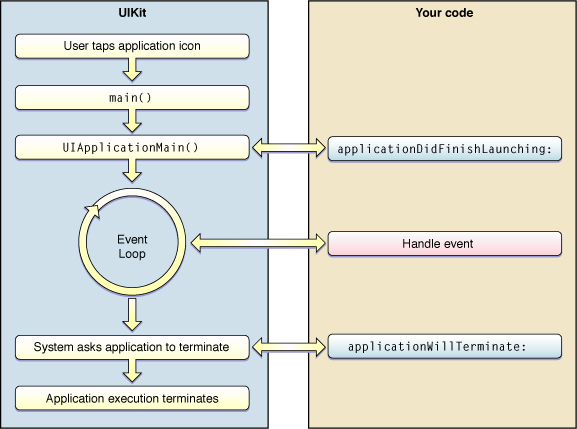
\includegraphics[width=0.8\textwidth]{./images/app_life_cycle.jpg}
  \caption{Ciclo de una aplicación iOS }
  \label{fig:iOS-layers}
\end{figure}
     
   La figura \ref{fig:iOS-layers} %\fxnote{incluir la referencia a la figura: \ref{fig:iPhoneOS layers}}
    muestra el ciclo de una aplicación para iOS. Tal y como vemos, UIKit se encarga del arranque de la aplicación y de la gestión de eventos. Nuestro código será el encargado de gestionar esos eventos justo cuando reciba la notificación de que la aplicación ha sido lanzada. También podremos gestionar las accionas oportunas (guardar preferencias o cambios producidos en la aplicación) cuando UIKit nos notifique la finalización de la aplicación.
   
    En iOS sólo se finaliza una aplicación por tres motivos:
    \begin{itemize}
	\item El usuario finaliza la misma pulsando el botón \textsf{Home}. %\fxnote{Yo usaría tipografía para el UI, por ejemplo \textsf{Home}.}.
	\item El sistema recibe una notificación prioritaria que atender (una llamada por ejemplo) y por tanto finaliza la aplicación. %\fxnote{Qué brusquedad! ¿realmente finaliza la aplicación? ¿no la suspende o algo parecido?}
	\item El sistema detecta un comportamiento erróneo de la aplicación y para salvaguardar la estabilidad del sistema finaliza nuestra aplicación.
     \end{itemize}

    Es responsabilidad del desarrollador asociar a cada evento un método adecuado para gestionarlo. Si el desarrollador deja un evento sin asociar, la aplicación simplemente lo ignorará.
    
%\fixme{Dudas que me surgen y que no se si este es el sitio o el momento adecuado para resolverlas. Lo que sí se es que impactan en el diseño: ¿qué eventos llegan al ``Your code''? ¿Qué reglas existen para tratarlos? ¿Se enlazan los eventos a métodos? ¿Se puede modificar ese supuesto ``vector de interrupciones''? ¿Los eventos son independientes de los objetos gráficos? Seguro que contestas a estas preguntas más adelante pero a mi, como lector, me gustaría saber algo más ahora.}    
    
\subsection{Controladores de Vista}	   

%\fxnote{¿Qué es una vista? ¿Te refieres a vistas del MVC o del SDK del iphone? ¿te refieres a controladores del MVC o del SDK?}
 
 Un controlador de vista del SDK proporciona la lógica básica de interfaz de usuario para dibujar las vistas de la aplicación. Definimos como vista de usuario la pantalla que se le presenta en un momento dado. Apple dispone de varios patrones de interfaces de usuario para ayudar a representar el conjunto de datos hacia el usuario en las aplicaciones dentro de los dispositivos móviles. 
 
  Un controlador de vistas gestiona la vista de nuestra aplicación que aparece entre las barras superiores e inferiores (véase figura \ref{fig:layout-of-views}).%\fxnote{\ref{fig:layout-of-views}}). 
  La vista de la aplicación aparece entre la barra de estado y la barra de navegación si ésta está presente. En una vista de aplicación se muestra una parte de datos y controles que el desarrollador quiere mostrar al usuario en un tiempo determinado. El controlador de la vista simplemente gestiona la presentación de esta vista y la siguiente en aparecer para un patrón de diseño establecido.
 
 \begin{figure} [h]
  \centering
    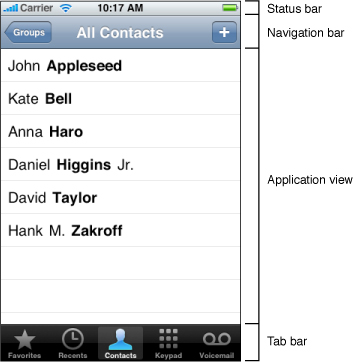
\includegraphics[width=0.8\textwidth]{./images/vc-areas.jpg}
  \caption{Esquema de las vistas }
  \label{fig:layout-of-views}
  %\fixme{Cuidado con los labels, no debes utilizar blancos aunque puedes usar ``:'' y ``-'' y ``\_''. de hecho empezar por fig: es una convención.}
\end{figure} 
 
 Usando controladores de vista eliminamos el código redundante e innecesario en las aplicaciones %\fxnote{¿en qué sentido?}
  y proporcionamos una interfaz de usuario familiar %\fxnote{¿familiar al ser usada por ``todos'' los programadores?}
  hacia los usuarios acostumbrados a la interfaz del terminal. %\fxnote{usuario-usuario}. 
 Los controladores de vista nos ahorran código al automatizar la presentación de cada vista al usuario. % \fxnote{¿Qué quieres decir?}. 
 También ayudan al diseño orientado de objetos separando los detalles de la interfaz de usuario de la lógica de la aplicación.
 
  Como ya hemos comentado los controladores de vista soportan el patrón de diseño MVC. %\fxnote{Pero\ldots ¿cómo funciona?}.
  Todos los datos y la lógica de la aplicación se ha implementado usando el lenguaje orientado a objetos emph{Objective-C}, para una mayor facilidad a la hora de la implementación haciendo uso de las herramientas del SDK.% \fxnote{Francisco, esta frase no dice nada, ¿de qué otra forma podrías implementarlos en ObjectiveC? ¿Donde están esos datos? ¿En las vistas? ¿En los controladores? ¿Donde está el modelo?}. 
  %En este caso los controladores de vista son los encargados de proporcionar los métodos delegados (métodos de la vista que delegan el control al controlador) %\fxnote{¿qué es un método delegado?}
   %y la fuente de datos para las vistas de tipo tabla que explicaremos a continuación.
  
 \subsection{Controlador Vista de tablas}	

  Es muy común usar vistas de tabla para mostrar un conjunto de datos de tipo jerárquico unido a los controladores de navegación para poder recorrerlos.  %\fxnote{¿Quieres decir que para implementar un modelo de datos jerárquico utilizas tablas + controladores de navegación? ¿qué es un controlador de navegación?}. 
  Para ello, disponemos % \fxnote{Yo evitaría utilizar tanto la palabra ``Apple'', puedes decir ``Para ello disponemos\ldots{}''.} dispone
   de una plantilla o ejemplo en las herramientas del SDK % \fxnote{¿Qué es una plantilla?} 
   de controlador llamada ``Controlador de vistas de tabla'' que nos proporciona todo lo necesario para ello. En nuestra aplicación, tenemos que mostrar el modelo de datos que recogemos de los servidores de Betfair. Éstos están organizados de forma jerárquica, de lo más general a lo más específico. Para poder realizar una apuesta en un partido de fútbol concreto antes hemos tenido que elegir deporte, categoría, país, división y finalmente el partido.
 La mejor forma de representarlos es mediante una vista de tabla tal y como nos recomiendan las hojas de estilo de Apple. Es la figura \ref{fig:table-view-top} podemos ver un esquema representativo de la información más general.

%\fixme{Creo que es muy importante resaltar esta justificación y para ello hemos de hablar antes del modelo de datos que impone Betfair.}
  
 \begin{figure}[h!]
  \centering
    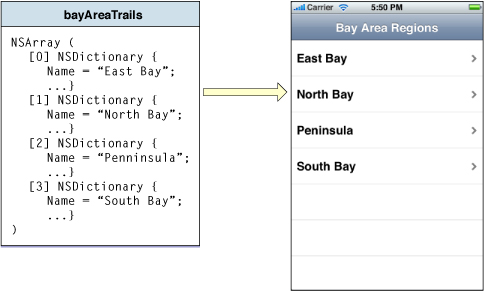
\includegraphics[width=0.7\textwidth]{./images/tv_datamodel_top.jpg}
  \caption{Vista de tabla del top de la jerarquía }
  \label{fig:table-view-top}
\end{figure} 

 En la figura \ref{fig:table-view-middle} nos encontramos una información de tipo jerárquica en la mitad de recorrido. Podemos asociarla al ejemplo de la elección de la división.

\begin{figure}[ht!]
  \centering
    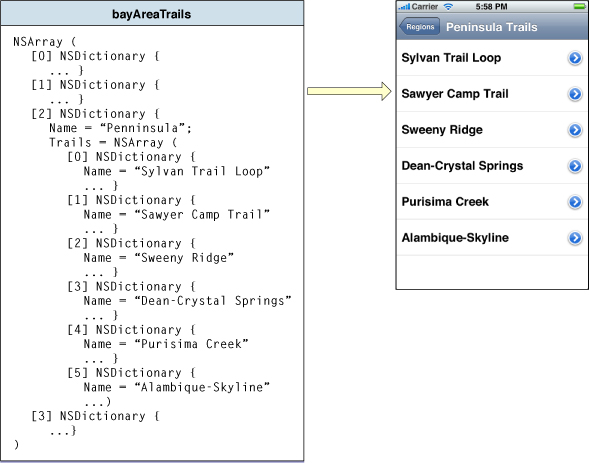
\includegraphics[width=0.7\textwidth]{./images/tv_datamodel_middle.jpg}
  \caption{Vista de tabla de la mitad de la jerarquía}
  \label{fig:table-view-middle}
\end{figure} 

 A continuación representamos el final de nuestro recorrido por el modelo de datos. Como podemos observar en la figura \ref{fig:detail-table-view}, hemos alcanzado la información más específica.

\begin{figure}[ht!]
  \centering
    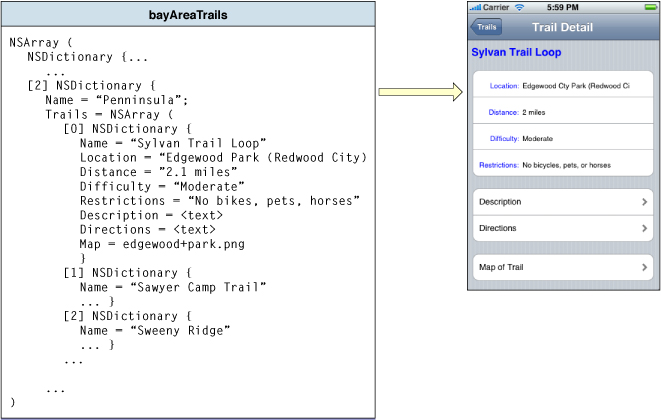
\includegraphics[width=0.8\textwidth]{./images/tv_datamodel_detail.jpg}
  \caption{Vista de tabla detallada del final de la jerarquía }
  \label{fig:detail-table-view}
\end{figure} 

%\fixme{Estas tres figuras así sueltas no aportan nada, tienes que explicar su significado y me parece superrelevante porque parece que con ello explicas cómo haces aparecer las listas en el iPhone.}

\subsection{Arquitectura de la aplicación}	
   
   Como ya hemos visto en apartados anteriores, la aplicación esta formada principalmente por un conjunto de controladores de vista más un módulo encargado de comunicarse con el API de Betfair. %\fixme{Fíjate que ésta es una decisión de diseño que aún no has explicado.}
   
   \begin{figure} [h]
     \centering
     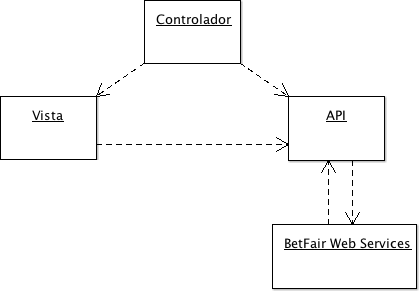
\includegraphics[width=0.8\textwidth]{./images/modelo1.png}
     \caption{Esquema modelo vista controlador }
     \label{fig:esquema-MVC}
   \end{figure}
   
    En la figura \ref{fig:esquema-MVC} podemos ver un esquema del modelo Vista Controlador usado. % \fxnote{de la arquitectura?}.
     Los controladores de vista se encargan de recoger los eventos de la aplicación, principalmente \emph{inputs} del usuario. % \fxnote{eventos?}. 
     En el caso de que el input involucre datos de Betfair, el controlador envía los datos necesarios para que el módulo de comunicación obtenga la respuesta por parte del API de Betfair. 
    
\subsubsection{Controlador principal}

 Es la clase principal de la aplicación. Es la encargada de iniciar el controlador de vista que será encargado de recoger los eventos del usuario, así como la gestión de memoria y la gestión de los eventos del sistema.
 
\subsubsection{Controlador de menú principal}
 Es la encargada de mostrar las opciones principales del programa y recoger los inputs del usuario para lanzar el controlador adecuado a la elección del usuario. También se encarga de gestionar el inicio de sesión del usuario para los servicios web de Betfair. Para ello hace uso del servicio \emph{login} de Betfair a través de la clase de comunicación llamada API.
 
\subsubsection{Controlador de tipos de eventos}
 Muestra al usuario una lista con todos los tipos de eventos activos por los que se puede apostar dentro de Betfair. En un futuro se podrá gestionar por fecha de finalización, orden alfabético o búsqueda directa de eventos. Una vez seleccionado el evento deseado, se lanza el controlador de eventos y mercados con la información relativa al evento previamente seleccionado. Hace uso del servicio de Betfair \emph{GetActiveEventsTypes}  a través de la clase API del modelo de la aplicación.
 
\subsubsection{Controlador de eventos y mercados}

 Es la clase encargada de mostrar de forma jerárquica los subeventos y mercados relacionados con un evento seleccionado previamente en el controlador de eventos. Igualmente se podrá gestionar por fecha de finalización, orden alfabético o búsqueda directa de eventos. En caso de ser seleccionado un evento, se le mostrará los mercados y subeventos relacionados con los mismos. Si se selecciona un mercado se procederá a lanzar el controlador de información de mercado. Para ello recaba la información obtenida a través del servicio web \emph{GetEvents} de Betfair.
 
\subsubsection{Controlador de información de mercado}

 Es el responsable de gestionar toda la información relevante al mercado en cuestión. Gestionará el estado del mercado y sus propiedades obteniendo todo lo necesario del portal de Betfair a través del API de sus servicios web haciendo uso de las llamadas del API:
 
  \begin{itemize}
	\item \emph{GetMarket}: obtiene todos los parámetros acerca del mercado.
	\item \emph{GetMarketPrices}: obtiene todos los precios actuales del mercado en cuestión.
\end{itemize}

\subsubsection{Controlador de apuesta por un mercado}
 Gestiona todos los datos necesarios e introducidos por el usuarios para realizar una apuesta y enviarla a Betfair. El método usado para enviar la apuesta a Betfair a través de la clase interfaz de comunicación es \emph{PlaceBets}.

\subsubsection{Controlador de las categorías de Mis Apuestas}
 Es la clase encargada de gestionar las apuestas ya realizadas en Betfair y que siguen activas. Las clasifica por categorías de mercado. Recoge la información como resultado de las llamadas a los siguientes servicios web de Betfair:
  \begin{itemize}
	\item \emph{GetMarket}: obtiene todos los parámetros acerca del mercado de una apuesta en cuestión.
	\item \emph{GetCurrentBets}: obtiene todas las apuestas realizadas por el usuario del servicios Betfair.
\end{itemize}
 
\subsubsection{Controlador de Mis Apuestas}
 Esta clase se encarga de gestionar las apuestas realizadas por el usuario dentro de una categoría determinada. En ella se muestra resumidamente el nombre de la apuesta en cuestión, la cuota apostada y la cuota actualizada en ese momento. 

\subsubsection{Controlador de detalles de una apuesta}
 Se encarga de gestionar todos los detalles sobre una apuesta determinada: parámetros, stake, apuesta a favor o en contra relacionadas con la presentada\ldots También incluye información completa del mercado actual referente al mercado de la apuesta y el trading acerca de la misma.

 
\subsubsection{API: Interfaz a Betfair}
 Esta clase se encarga de gestionar las comunicaciones con los servidores de Betfair. Envía las peticiones a los servicios web de Betfair y se encarga de realizar la decodificación de la respuesta a dichas peticiones en un formato adecuado para la aplicación.

\section{Diagrama de Clases}
 En la siguiente figura podemos ver el diagrama de clases del proyecto. Observamos que el núcleo de esta aplicación es la clase ``API". Como bien hemos descrito es la encargada de comunicarse con el servidor de Betfair tanto para enviar las peticiones como de procesar las respuestas. Esta clase necesita un \emph{parser} de XML para obtener los datos del mensaje de respuesta, de esta tarea se encarga la clase ``ParserXML''.
 
  A partir de ahí observamos que le rodean todos los controladores de vista de la aplicación, ya que son los que reciben las peticiones de la vista y la envían a la clase ``API''. ``RootViewController'' es la clase principal. Se lanza cuando se carga la aplicación y es la encargada de procesar el menú de la misma.

 \begin{figure}[h!]
    \centering
       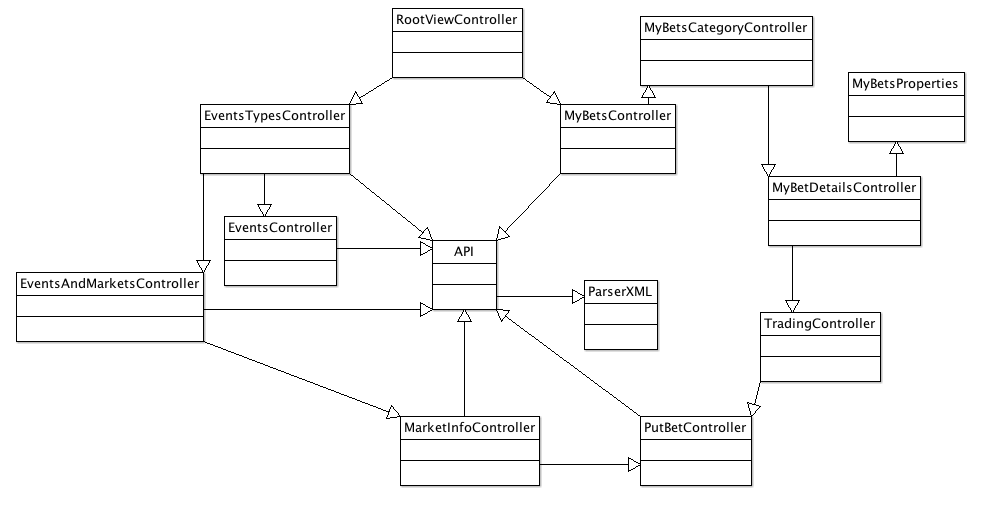
\includegraphics[width=1.2\textwidth]{./images/DiagramaDeClases3.png}
     \caption{Diagrama de clases}
   \label{fig:Diagrama de clases}
\end{figure}

%%% Local Variables: 
%%% mode: latex
%%% TeX-master: "tfc-betfair-ios"
%%% TeX-PDF-mode: t
%%% ispell-local-dictionary: "castellano"
%%% End: 
